\documentclass[11pt]{article}
\usepackage[polish]{babel}
\usepackage[T1]{fontenc}
\usepackage{hyperref}
\usepackage{array}
\usepackage{amssymb}
\usepackage{amsmath}
\usepackage{changepage}
\usepackage{multicol}
\usepackage{listings}
\usepackage{xcolor}
\hypersetup{
    colorlinks,
    citecolor=black,
    filecolor=black,
    linkcolor=black,
    urlcolor=black
}
\usepackage{graphicx}

\usepackage{tikz}
\usetikzlibrary{fit,arrows,matrix,positioning, calc, shapes.gates.logic.IEC, shapes.gates.logic.US}
\usetikzlibrary {arrows.meta}
\tikzstyle{branch}=[fill,shape=circle,minimum size=3pt,inner sep=0pt]

\usepackage{geometry}
\geometry{a4paper, portrait, margin=1in}

\definecolor{codegreen}{rgb}{0,0.6,0}
\definecolor{codegray}{rgb}{0.5,0.5,0.5}
\definecolor{codepurple}{rgb}{0.58,0,0.82}
\definecolor{backcolour}{rgb}{0.95,0.95,0.92}

\lstdefinestyle{mystyle}{
    backgroundcolor=\color{backcolour},   
    commentstyle=\color{codegreen},
    keywordstyle=\color{magenta},
    numberstyle=\tiny\color{codegray},
    stringstyle=\color{codepurple},
    basicstyle=\ttfamily\footnotesize,
    breakatwhitespace=false,         
    breaklines=true,                 
    captionpos=b,                    
    keepspaces=true,                 
    numbers=left,                    
    numbersep=5pt,                  
    showspaces=false,                
    showstringspaces=false,
    showtabs=false,                  
    tabsize=4
}

\lstset{style=mystyle}

\title{%
        \vspace{-1cm}
       \large Optymalizacja Kombinatoryczna - Projekt \\
       \huge  Ant System dla problemu komiwojażera}

\author{Michał Łatka 160263 \\ Stanisław Fiedler 160250}
\date{Politechnika Poznańska, Styczeń 2025}

\begin{document}


\maketitle
\tableofcontents

\section{Ant System}\label{sec:ant_system} % (fold)

\subsection{Inicjalizacja}\label{sub:inicjalizacja} % (fold)
Instancja początkowa reprezentowana jest przez następujące dane: liczbę wierzchołków $(n)$ oraz n par liczb całkowitych $(x_i, y_i)$ oznaczających rozmieszczenie tych wierzchołków na płaszczyźnie kartezjańskiej.
\begin{center}
	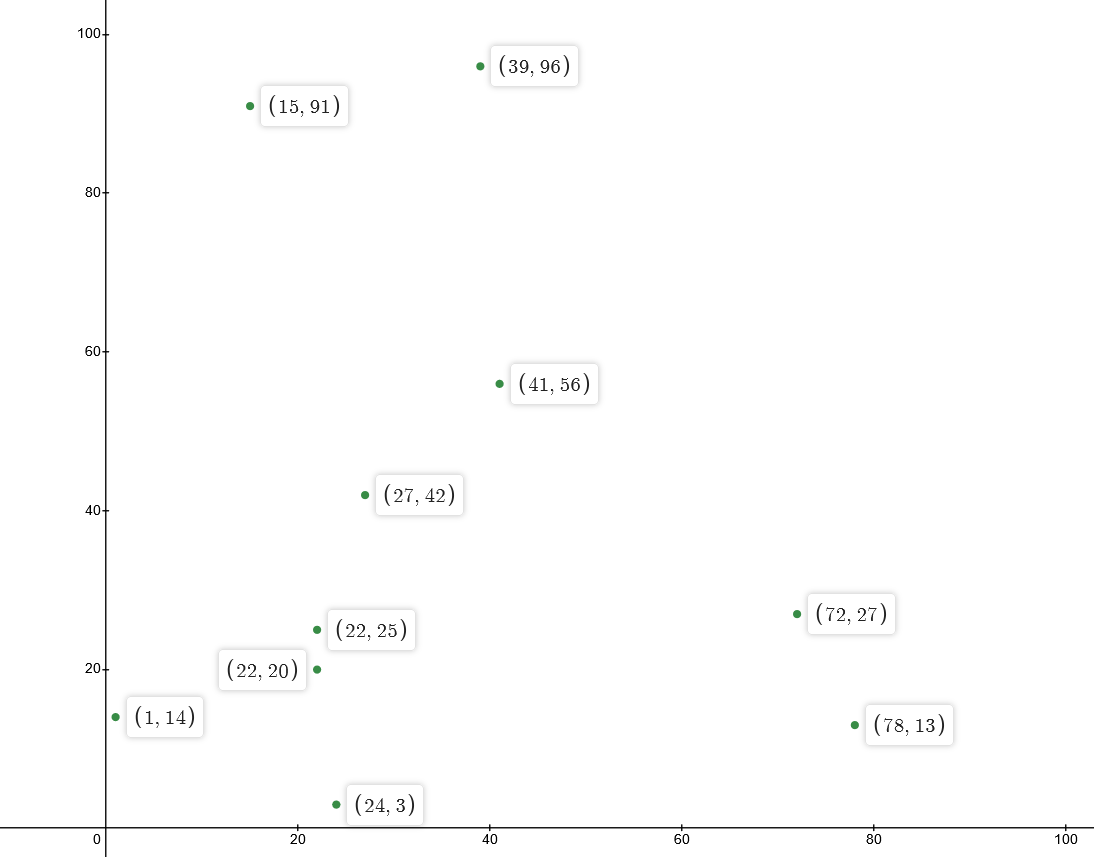
\includegraphics[scale=0.3]{images/init.png}
\end{center}

% subsection Inicjalizacja (end)

\subsection{Opis Algorytmu}\label{sub:opis_algorytmu} % (fold)
Algorytmy mrówkowe są stosowane przy rozwiązywaniu niektórych problemów NP-trudnych.
W przeszukiwaniu przestrzeni rozwiązań symulują one zachowanie kolonii mrówek.
Każde znalezione rozwiązanie pozostawia informacje używane do budowy następnego.

Dla problemu komiwojażera w każdej iteracji wypuszczana jest pewna ilość mrówek które mają znaleźć rozwiązanie.
Dla każdej mrówki, po znalezieniu ścieżki, na każdej krawędzi z której jest zbudowana, jest dodawana wartość (tzw. feromony) odwrotnie proporcjonalna do długości znalezionego rozwiązania.
Mrówka tworząc trasę wybiera wierzchołki z prawdopodobieństwem zgodnym z siłą feromonów na krawędziach.
Po każdej iteracji z krawędzi jest usuwany pewien procent feromonów.

Działanie algorytmu jest zależne od ustawionych parametrów:
\begin{description}
	\item INITIAL\_FEROMONES: początkowa wartość feromonów na krawędziach
	\item EVAPORATION\_RATE: ułamek feromonów usuwany przy każdej iteracji
	\item Q: stała określająca ilość feromonów pozostawianych przez mrówki
	\item A, B: stałe używane przy wyborze następnego wierzchołka
\end{description}
% subsection Opis Algorytmu (end)

\subsection{Pseudokod}\label{sub:pseudokod} % (fold)

\lstinputlisting[language=c++]{../pseudokod.txt}

% subsection Pseudokod (end)

\pagebreak
\subsection{Przykład obrazujący działanie}\label{sub:przyklad} % (fold)
Intensywność feromonów na krawędziach po 1 iteracji:\\
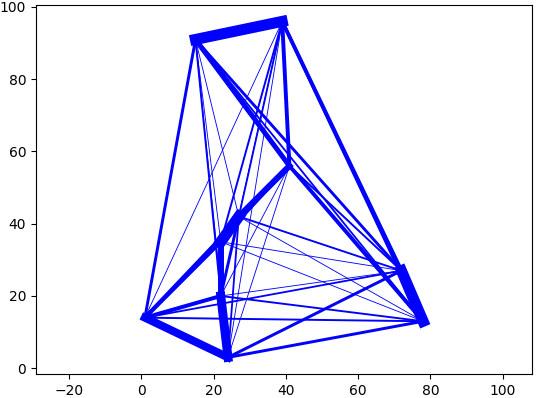
\includegraphics[scale=0.5]{images/fer1.png}


Intensywność feromonów na krawędziach po 2 iteracjach:\\
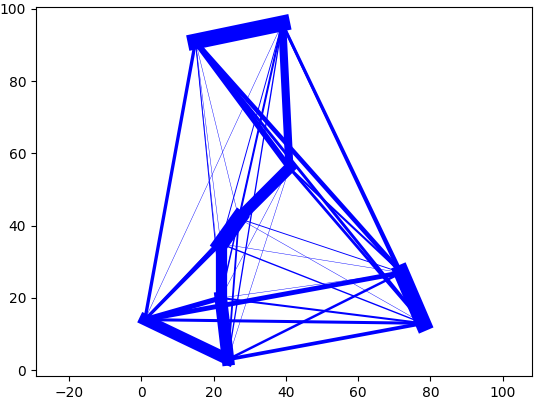
\includegraphics[scale=0.5]{images/fer2.png}


Intensywność feromonów na krawędziach po 5 iteracjach:\\
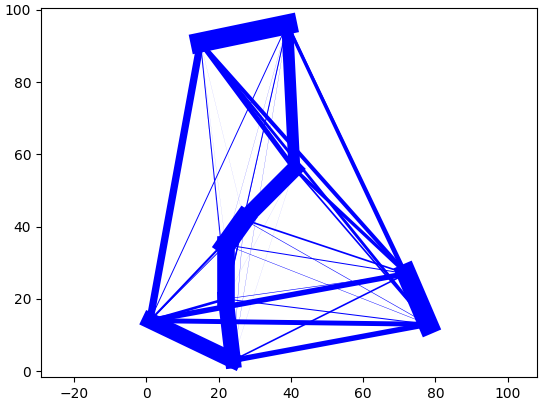
\includegraphics[scale=0.5]{images/fer3.png}
% subsection przyklad (end)

\subsection{Finalizacja}\label{sub:finalizacja} % (fold)
Intensywność feromonów na krawędziach po zakończeniu programu:\\
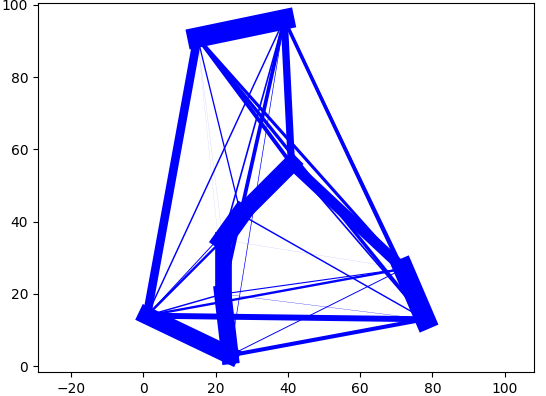
\includegraphics[scale=0.5]{images/fer_res.png}

Najkrótsza znaleziona ścieżka (długości 298.551 j):\\
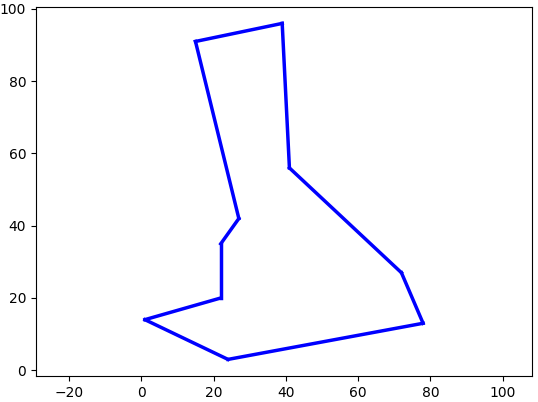
\includegraphics[scale=0.5]{images/path.png}
% subsection Finalizacja (end)

% section Ant System (end)

\section{Wykresy}\label{sec:wykresy} % (fold)

\subsection{Porównanie z algorytmem zachłannym}\label{sub:} % (fold)
Porównanie optymalizowanej wartości dla algorytmu Ant System z algorytmem zachłannym:\\
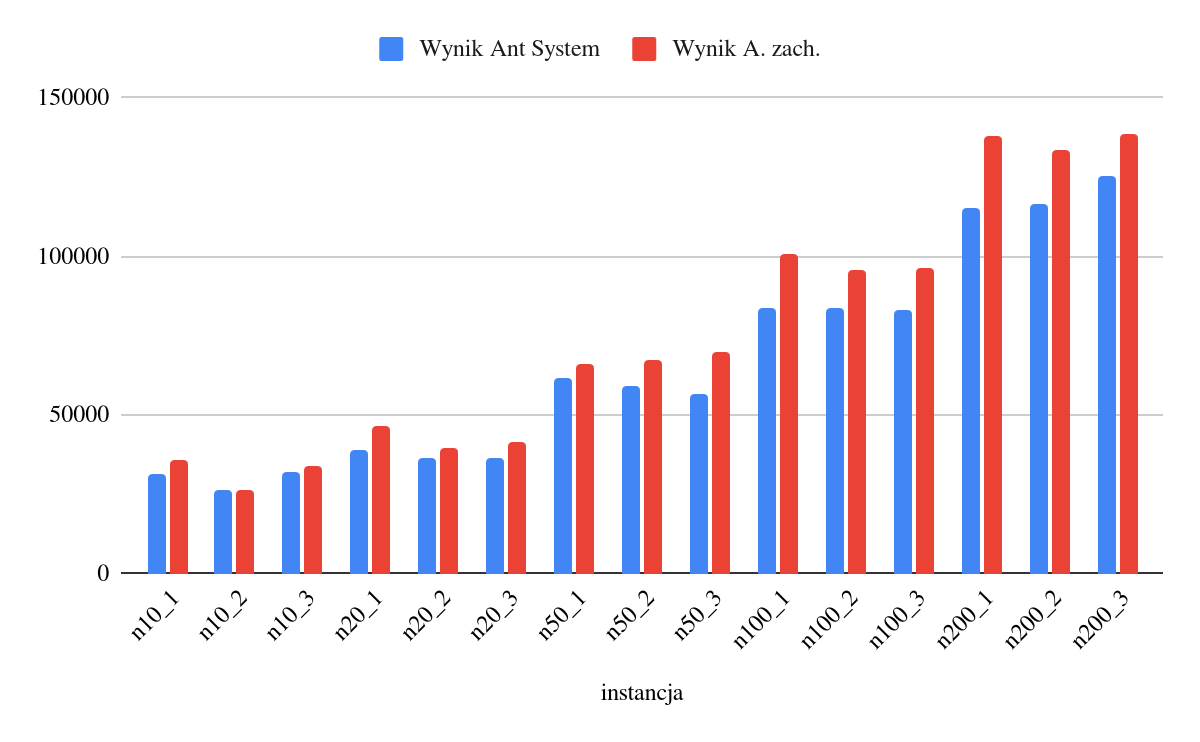
\includegraphics[scale=0.35]{images/greedy.png}
% subsection  (end)

\subsection{Wartości błędu do wartości optymalnej}\label{sub:blad} % (fold)
Wykres wartości błędu względnego algorytmu Ant System w stosunku do wartości optymalnej:\\
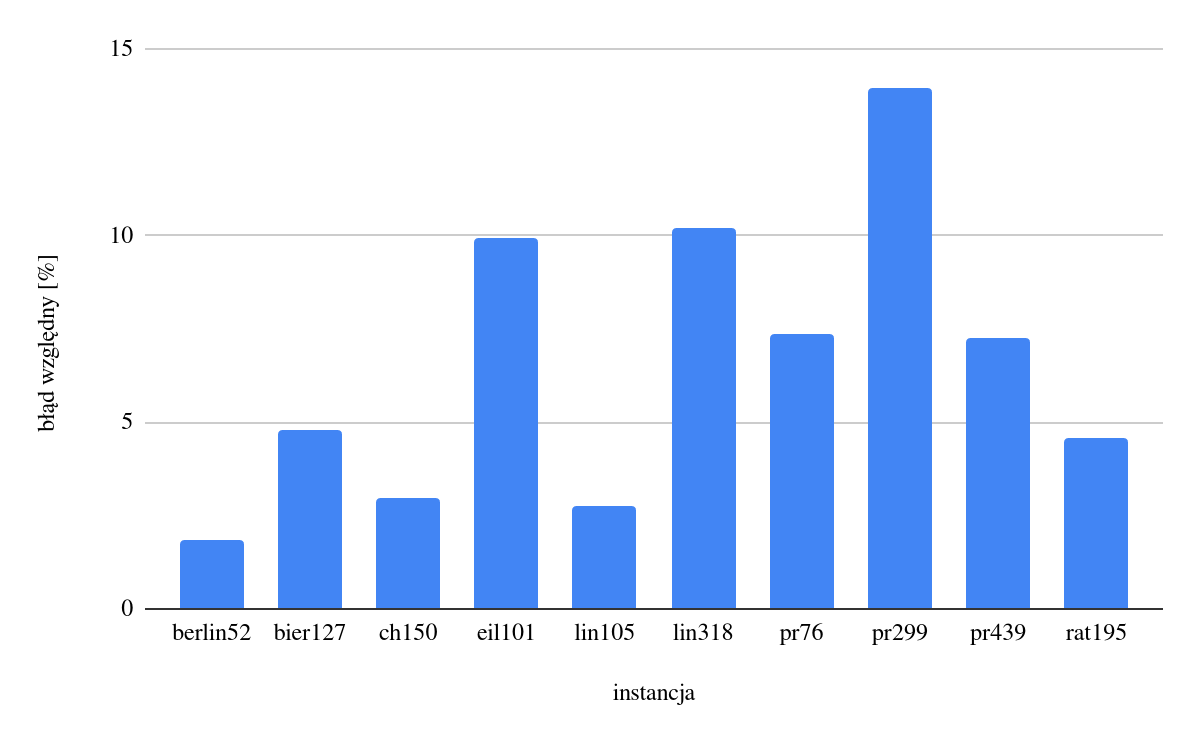
\includegraphics[scale=0.35]{images/error.png}
% subsection blad (end)

\subsection{Wyniki algorytmu dla instancji rankingowych}\label{sub:wyniki_algorytmu_dla_instancji_rankingowych} % (fold)
\begin{center}
	\Large
	\begin{tabular}{c | c}
		\textbf{Nazwa instancji} & \textbf{Wynik} \\
		\hline\hline
		berlin52                 & 7677           \\ \hline
		bier127                  & 123903         \\ \hline
		tsp250                   & 13414          \\ \hline
		tsp500                   & 93377          \\ \hline
		tsp1000                  & 27362
	\end{tabular}
\end{center}

% subsection Wyniki algorytmu dla instancji rankingowych (end)

% section Wykresy (end)

\end{document}

